\begin{figure}[t]
    \centering
    % \begin{subfigure}[t]{0.25\textwidth}
    %     \centering
    %     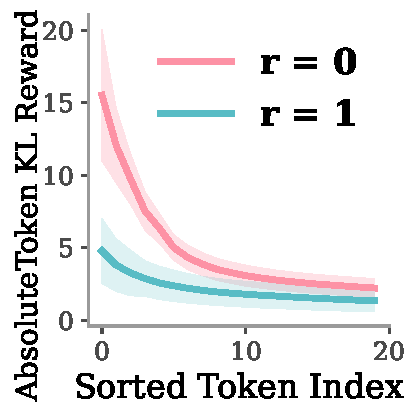
\includegraphics[width=\linewidth]{figures/token_rewards_correct_vs_incorrect.pdf}
    %     \captionsetup{width=0.9\linewidth}
    %     \caption{}
    %     \label{fig:credit-assignment-a}
    % \end{subfigure}
    % \hfill
    % \begin{subfigure}[t]{0.73\textwidth}
    %     \centering
    %     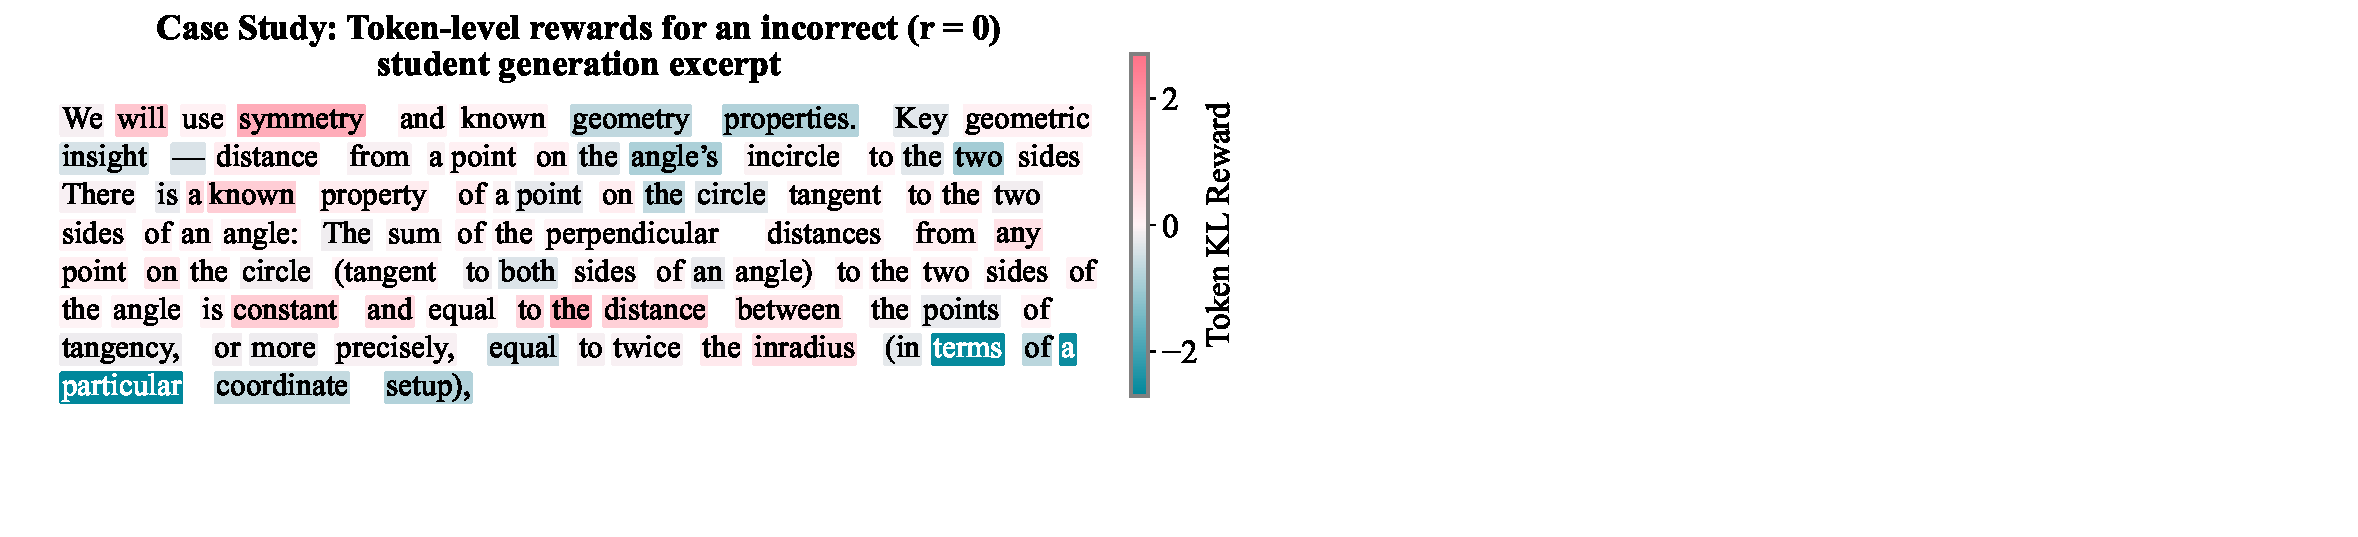
\includegraphics[
    %         width=\linewidth,
    %         trim=0.5cm 2cm 19cm 0cm,
    %         clip
    %     ]{figures/sample_9013_excerpt_token_reward_heatmap.pdf}
    %     \captionsetup{width=0.9\linewidth}
    %     \caption{}
    %     \label{fig:credit-assignment-b}
    % \end{subfigure}
    \captionsetup{font=small}
    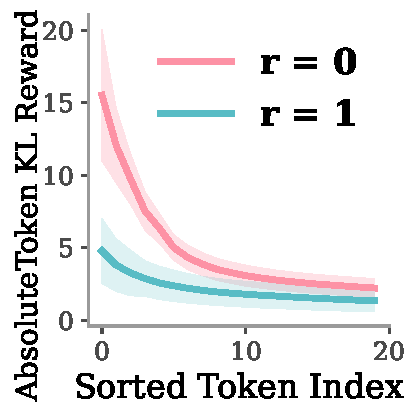
\includegraphics[width=0.25\textwidth]{figures/token_rewards_correct_vs_incorrect.pdf}
    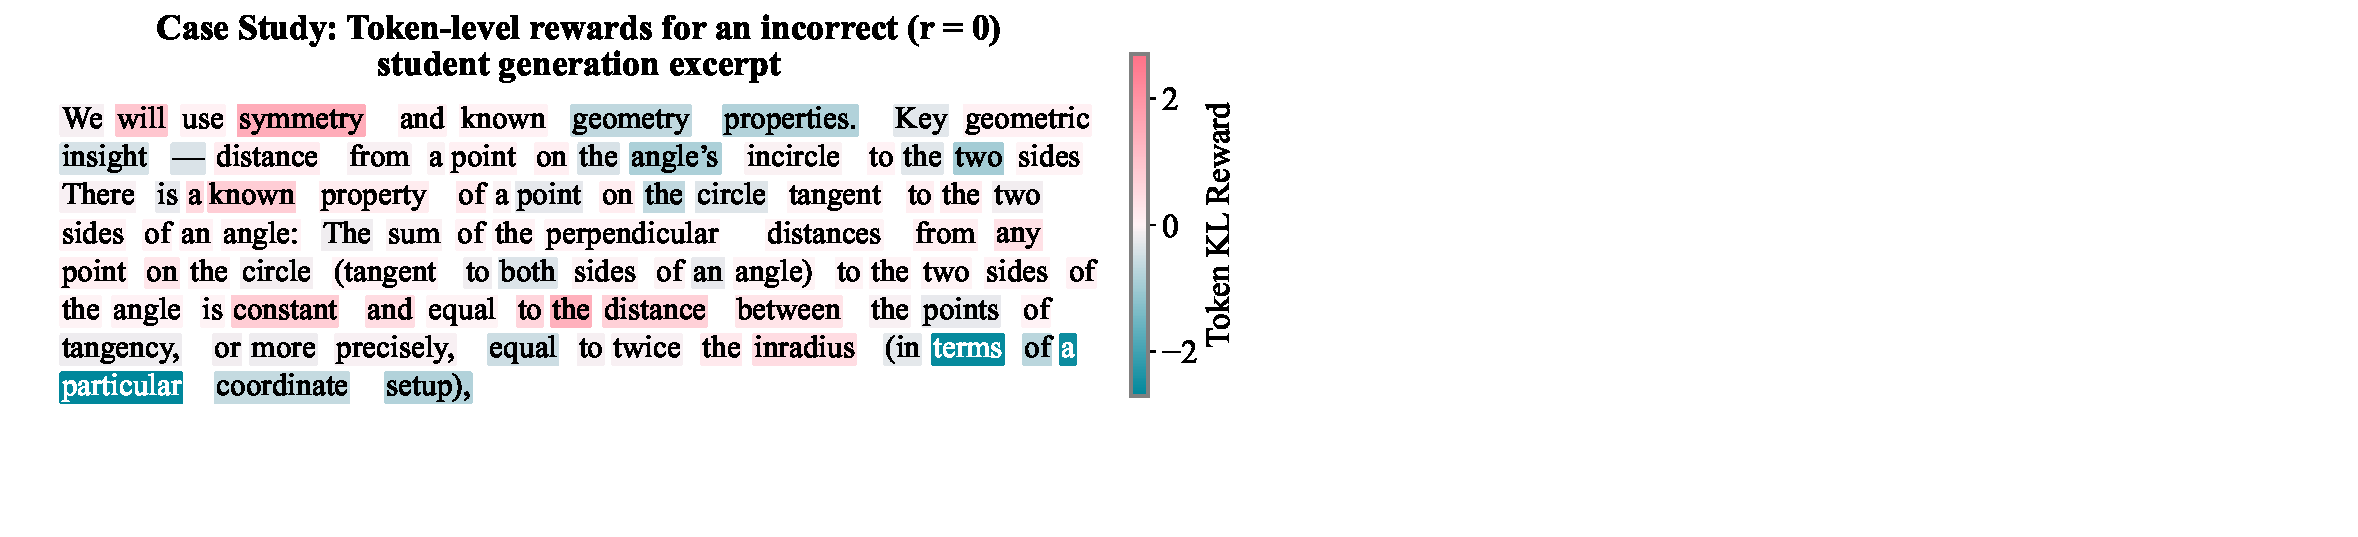
\includegraphics[
            width=0.73\textwidth,
            trim=0.5cm 2cm 19cm 0cm,
            clip
        ]{figures/sample_9013_excerpt_token_reward_heatmap.pdf}
    \caption{\looseness-1\textbf{Reviser converts binary outcome reward into dense token-level reward.}
\textbf{Left:} Comparison of token-level KL reward distributions for correct (\(\mathbf{r=1}\)) and incorrect (\(\mathbf{r=0}\)) student generations.
Incorrect trajectories concentrate larger rewards on a small number of tokens, whereas correct trajectories receive a flatter reward distribution that mainly preserves the response.
\textbf{Right:} Visualization of token-level KL rewards for an incorrect student generation (\(\mathbf{r=0}\)).
The teacher policy converts binary reward \(r=0\) to dense rewards that localize mistake-relevant tokens and guide targeted correction. 
}
    \vspace{-10pt}
    \label{fig:credit-assignment}
\end{figure}
